\chapter{Experimentos}
\label{cap:experiments}

\section{Ambiente de simulação}

Uma simulação da rede nacional de pesquisa, a rede Ipê \citep{ipe2015network} 
foi criada em laboratório.
Um comutador (\emph{switch}) OpenFlow e quatro servidores foram utilizados 
para executar a simulação no laboratório WiNet \citep{winet22015lab}
no departamento de Ciência da Computação (DCC) da Universidade Federal 
de Minas Gerais (UFMG).

\subsection{A rede Ipê}
Operada pela Rede Nacioanal de Pesquisa (RNP), a rede Ipê é uma infraestrutura
de rede Internet dedicada à comunidade de pesquisa brasileira.
Inaugurada em 2005, foi a primeira rede óptica nacional acadêmica a entrar em
operação na América Latina.

A rede IPÊ implementa 27 Pontos de Presença (\emph{POPs}), um para cada unidade
da federação.
Em cada unidade existem diversos clientes que, para se comunicar com outras 
máquinas em outros Pontos de Presença, transmitem seus pacotes através do 
POP ao qual atuam como clientes.
Essas ramificações constituem mais de 800 instituições de ensino, saúde e 
pesquisa em todo o país, beneficiando mais de 3,5 milhões de usuários
\citep{ipe2015network}.

Através da rede RedCLARA \citep{redclara2015network}, a rede Ipê se conecta 
à 2,5 Gb/s com, atualmente, 15 países da América Latina e à 5 Gb/s com a rede
europeia Géant \citep{geant2015network}. 
Além disso, por meio de quatro conexões de
10 Gb/s, duas pelo Oceano Atlântico e duas pelo Oceano Pacífico, 
operadas em parceria com a ANSP, totalizando 40 Gb/s, a rede Ipê se conecta 
às redes acadêmicas norte-americanas, em especial, a  Internet2 
\citep{internet22015network}, a outras redes acadêmicas internacionais e à 
internet comercial mundial.

Os Pontos de presença estão interconectados conforme mostrado na figura 

\ref{fig:ipe-network-2015}.

\begin{figure}[!h]
    \centering
    \label{fig:ipe-network-2015}
    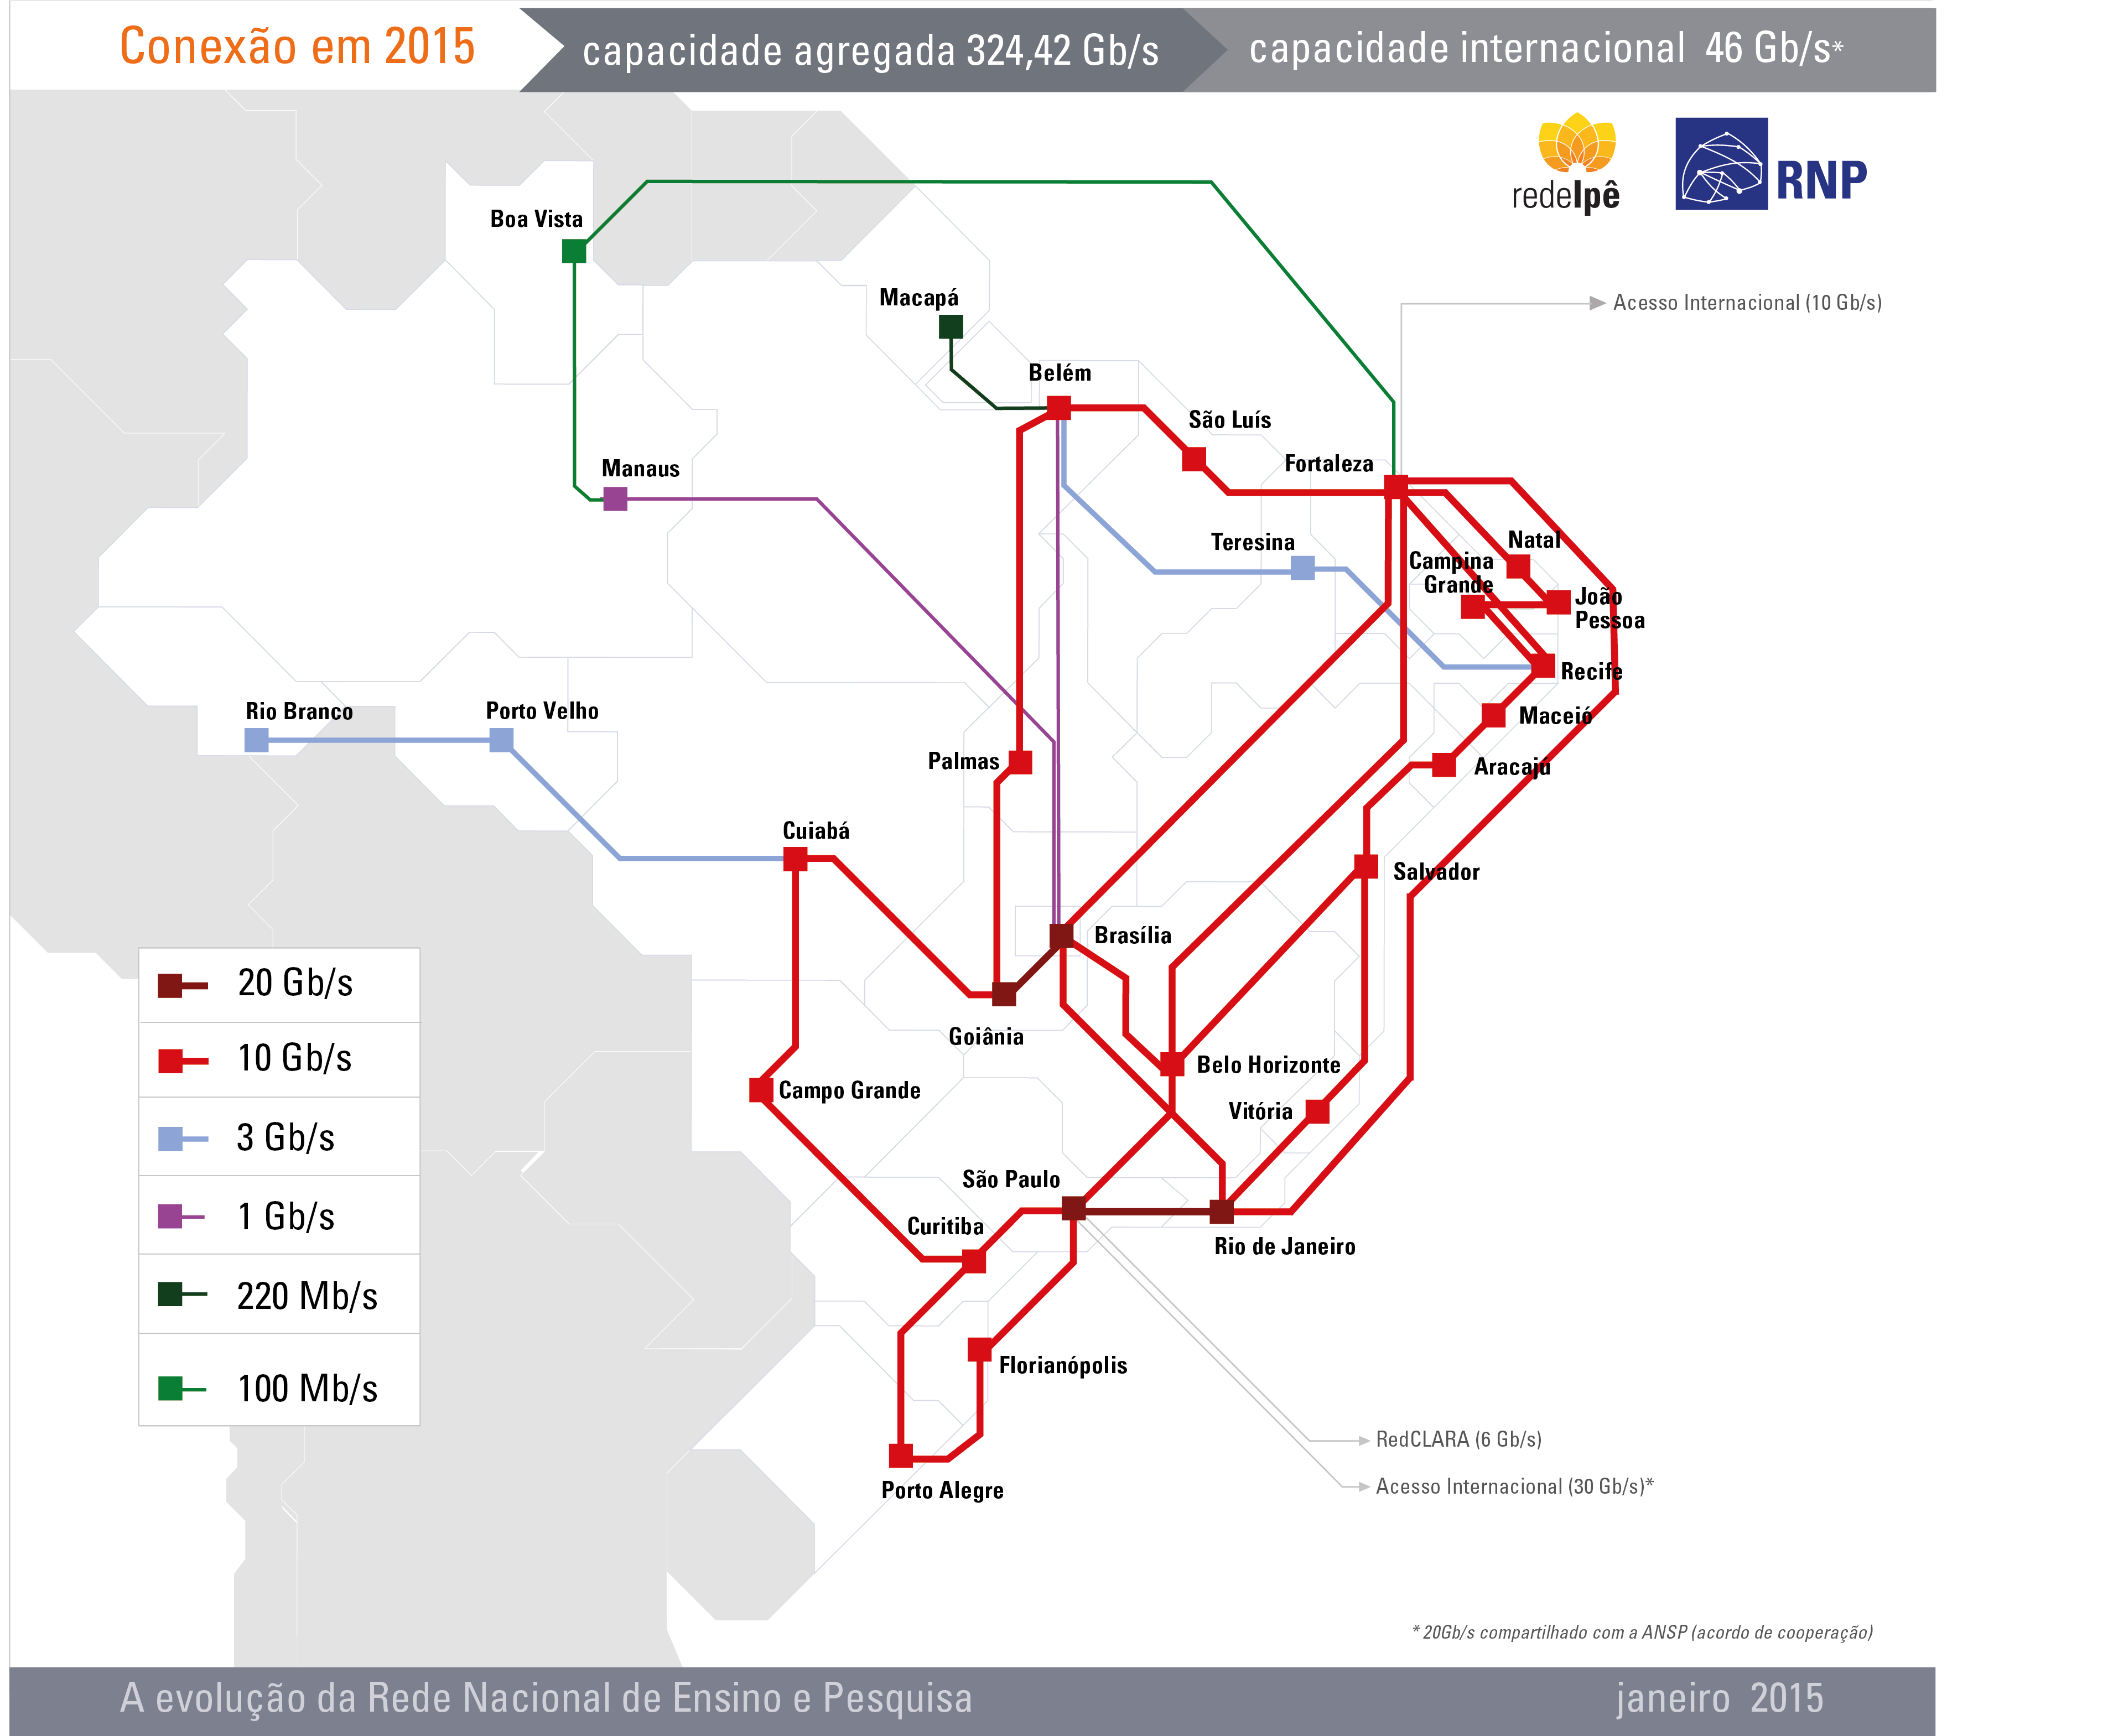
\includegraphics[width=\linewidth]{img/ipe-network-2015}
    \caption{Rede Nacional de Pesquisa IPÊ \protect\footnotemark}
\end{figure}

\footnotetext{Imagem retirada de 
\url{http://www.rnp.br/servicos/conectividade/rede-ipe}}

\subsection{Arquitetura da simulação}


\begin{table}[h]
    \label{tbl:testbed-ipe-net}
    \centering
    \resizebox*{!}{\dimexpr\textheight- 25px}{
    \resizebox{\linewidth}{!}{
    \begin{tabular}{llllll}
        \rowcolor[HTML]{000000} 
        \multicolumn{6}{c}{\cellcolor[HTML]{000000}{\color[HTML]{C0C0C0} 
            \textbf{Associação de Servidores à simulação da rede IPÊ}}} \\
        \rowcolor[HTML]{000000} 
        {\color[HTML]{9B9B9B} \textbf{UF}} & {\color[HTML]{9B9B9B} 
            \textbf{N clientes}} & {\color[HTML]{9B9B9B} 
            \textbf{Sub-rede local}} & {\color[HTML]{9B9B9B} 
            \textbf{Servidor}} & {\color[HTML]{9B9B9B} \textbf{IP local}} & 
            {\color[HTML]{9B9B9B} \textbf{IP Gateway}} \\
        AC &  10 &  10.10.1.0 &   Shiva  &  10.10.42.51 & \\ 
        AL  & 13 &  10.10.2.0  &  Shiva  &  10.10.42.52 & \\ 
        AM  & 20 &  10.10.3.0 &   Shiva  &  10.10.42.53 & \\
        AP  & 7  &  10.10.4.0 &   Shiva  &  10.10.42.54 & 10.10.42.50 \\
        BA  & 25 &  10.10.5.0 &   Shiva  &  10.10.42.55 & \\
        CE  & 50  & 10.10.6.0  &  Shiva  &  10.10.42.56 & \\
        DF  & 16 &  10.10.7.0  &  Shiva  &  10.10.42.57 & \\ \hline
        ES  & 26  & 10.10.8.0  &  Eden  &   10.10.42.101 & \\
        GO  & 26  & 10.10.9.0  &  Eden  &   10.10.42.102  & \\  
        MA  & 7  &  10.10.10.0 &  Eden  &   10.10.42.103  & \\  
        MG  & 32  & 10.10.11.0  & Eden  &   10.10.42.104  & 10.10.42.100 \\  
        MS  & 10  & 10.10.12.0  & Eden  &   10.10.42.105  & \\  
        MT  & 8   & 10.10.13.0  & Eden  &   10.10.42.106  & \\  
        PA  & 13  & 10.10.14.0  & Eden  &   10.10.42.107  & \\ \hline
        PB  & 14  & 10.10.15.0  & Diablos & 10.10.42.151  & \\
        PE  & 41  & 10.10.16.0  & Diablos & 10.10.42.152  & \\  
        PI &  25 &  10.10.17.0 &  Diablos & 10.10.42.153  & \\  
        PR &  71 &  10.10.18.0 &  Diablos & 10.10.42.154  & 10.10.42.150 \\
        RJ &  27 &  10.10.19.0 &  Diablos & 10.10.42.155  & \\  
        RN &  11 &  10.10.20.0 &  Diablos & 10.10.42.156  & \\  
        RO &  10 &  10.10.21.0 &  Diablos & 10.10.42.157  & \\ \hline
        RR  & 7  &  10.10.22.0 &  Leviathan &   10.10.42.201 & \\
        RS &  10 &  10.10.23.0 &  Leviathan &   10.10.42.202  & \\  
        SC &  47 &  10.10.24.0 &  Leviathan &   10.10.42.203 & 10.10.42.200 \\   
        SE &  13 &  10.10.25.0 &  Leviathan &   10.10.42.204 & \\   
        SP &  25 &  10.10.26.0 &  Leviathan &   10.10.42.205  & \\  
        TO &  11 &  10.10.27.0 &  Leviathan &   10.10.42.206 & \\   
    \end{tabular}
    }}
\end{table}


\section{Detecção de entidades}

\section{Remoção de entidades}

\section{Visualização em tempo real}

\section{Identificação de tráfego}

\section{Rede Nacional de Pesquisa (RNP-IPÊ)}
